% title: Dead code elimination removes unused equations
% description: The original IR contains a used equation and an unused equation. DCE removes the unused equation while retaining the equation needed for the selected output.
\documentclass[tikz,border=5pt]{standalone}
\usetikzlibrary{arrows.meta,calc,shapes.geometric}
\definecolor{numeric}{HTML}{4477AA}
\definecolor{textual}{HTML}{AA4499}

\tikzset{
    box/.style={draw, line width=0.8pt, minimum height=0.8cm,
                minimum width=1.8cm, inner sep=6pt, align=center},
    ir/.style={box},
    flow/.style={-{Stealth[length=5pt]}, line width=0.9pt},
    feedback/.style={flow, dashed},
    note/.style={font=\small, align=center},
    choice/.style={diamond, draw, line width=0.8pt,
                   aspect=2, inner sep=2pt, align=center},
}

\newcommand{\irframe}[2]{
    \draw[line width=0.8pt] #1 rectangle #2;
}

\newcommand{\transformarrow}[4][above]{
    \draw[flow] (#2) -- node[#1=6pt,note] {#4} (#3);
}


\tikzset{
    transform panel/.style={font=\small},
    transform program/.style={ir, minimum width=2.8cm},
}

\newcommand{\transformcanvas}{
    \path[use as bounding box] (-6.6,-2.75) rectangle (6.6,2.65);
}

\begin{document}
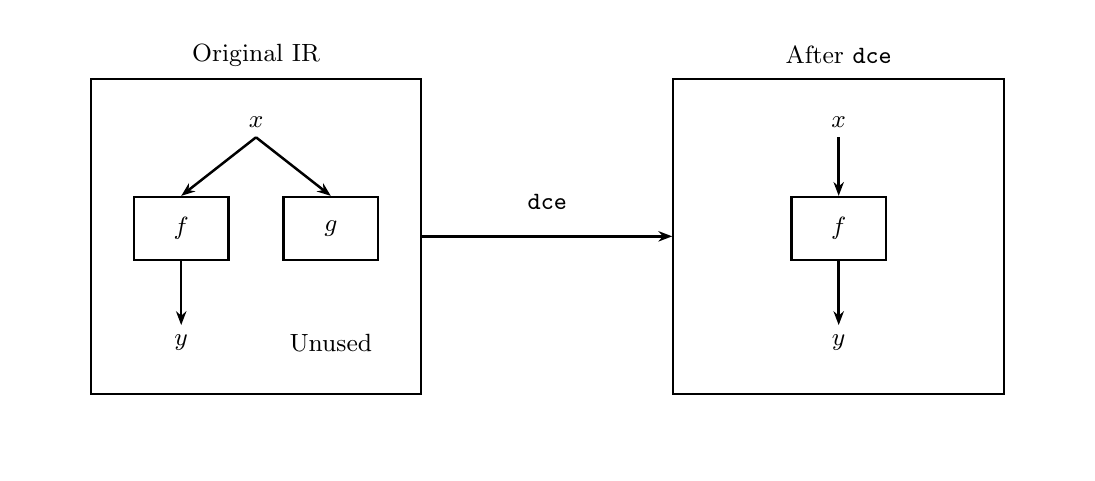
\begin{tikzpicture}[transform panel]
    \transformcanvas

    \node[ir, minimum width=4.2cm, minimum height=4cm] (original) at (-3.7,0) {};
    \node at (-3.7,2.3) {Original IR};
    \node (input) at (-3.7,1.45) {$x$};
    \node[box, minimum width=1.2cm] (used) at (-4.65,0.1) {$f$};
    \node[box, minimum width=1.2cm] (unused) at (-2.75,0.1) {$g$};
    \node (output) at (-4.65,-1.35) {$y$};
    \node at (-2.75,-1.35) {Unused};
    \draw[flow] (input.south) -- (used.north);
    \draw[flow] (input.south) -- (unused.north);
    \draw[flow] (used.south) -- (output.north);
    \node[ir, minimum width=4.2cm, minimum height=4cm] (new) at (3.7,0) {};
    \node at (3.7,2.3) {After \texttt{dce}};
    \node (newin) at (3.7,1.45) {$x$};
    \node[box, minimum width=1.2cm] (kept) at (3.7,0.1) {$f$};
    \node (newout) at (3.7,-1.35) {$y$};
    \draw[flow] (newin.south) -- (kept.north);
    \draw[flow] (kept.south) -- (newout.north);
    \transformarrow{original.east}{new.west}{\texttt{dce}}

\end{tikzpicture}
\end{document}
